\section{Mobile CI/CD}

Coming now from the "classical" CI/CD approach, it is not possible to instantly apply the known model to the mobile world, it needs some adoption. Before we do so, we have to consider the following points: \\

\begin{itemize}
	
	\item \textbf{Mobile application have a high UI focus} \\
	UI tests are always more expensive to create than for "standard" code - and this is even more valid for mobile applications. Additionally from the known challenges of desktop applications like clickable fields, listener states, dependencies between views \& co, a mobile device introduces complexity
	\\
	
	\item \textbf{Mobile applications have per default a build tool} \\
	Both iOS (\textit{XCode}) and Android (\textit{AndroidStudio} \& \textit{gradle}) come along with their own build system and IDE, making the question if the application is build manually or automated with a tool pointless.
	\\
	
	\item \textbf{There is no standard production environment} \\
	Due to the nature of the mobile device world, there is no standard device towards a deployment can happen. Especially but not only with Android there is a huge variety of screen sizes and operating system versions to be handled. Therefore automated testing has to be a compromise between covered variations and invested efforts. There are of course attempts to test with assuming the maximum coverage of variations, but it can never be sufficient as for e.g. a server software.
	\\
	
	\item \textbf{Emulation is expensive} \\
	Another consequence of the variety of device types, testing with real hardware is a pain and lead to the usage of emulators. But emulation is expensive in terms of time and resources, especially since due to the high share of required UI tests, a majority of testing can not be done independent from the (emulated) mobile OS.
	
\end{itemize}

\subsection{Adopted CI/CD model}
As consequence to the mentioned points, we will adopt the practise checklist of Fowler by completely removing 2) (inherited to the build tools) and changing 7) to "Test in a Emulated Environment".

\subsection{Googles CI/CD tools}

Google provides many frameworks and guidelines which can be pretty overwhelming - this and the next section is therefore dedicated to give an overview of these and summarize which options there are to implement a proper CI/CD pipeline within the Android world. 

\subsubsection{Android Emulator}

Bundled within the Android SDK comes the Android Emulator\footnote{\url{https://developer.android.com/studio/run/emulator}}, which allows the emulation of a virtual device on the local machine. It supports various images, called Android Virtual Devices (AVD), with different configuration options. Once launched it is considered as a real device by \texttt{adb} and can therefore used as deployment target. The tool further provides the option to launch without an UI and to be used for testing on a server.

\subsubsection{Firebase Test Lab}
With Firebase Test Lab\footnote{\url{https://firebase.google.com/docs/test-lab/android/overview}} Google offers a cloud-based device farm with virtual and real devices. It supports two different testing methods: Instrumentation (see section~\ref{sec:test_types}) and Robo (basic test type that simulates real user interactions) Tests. Test results are provided with additional logs, videos and screenshots.
Firebase Test Lab allows 10 tests per day for virtual devices and 5 for physical devices in it's free version ("Spark Plan") - but some CI/CD cloud services like Bitrise included the service within their contingents.

\subsubsection{Google Play Deploy}
Google offers via the Play Store console a REST API to deploy compiled APKs and AABs which can be used in an CD setup. The API is secured via the according Service account. Additionally to the (not prefered way) direct release track it is possible to deploy to the \texttt{alpha}, \texttt{beta} or \texttt{internal} tracks\footnote{\url{https://developers.google.com/android-publisher/tracks}}.

\subsubsection{Available CI/CD Server}

In order to properly utilize a mobile CI/CD pipeline there are many estabilshed server provider around - since it would exceed the scope of this paper to make a full comparison of these service providers, we limit it to a selection of the most commons:

\begin{itemize}
	\item Bitrise\footnote{\url{https://www.bitrise.io/}}
	\item TeamCity\footnote{\url{https://www.jetbrains.com/teamcity/}}
	\item Travis CI\footnote{\url{https://travis-ci.org/}}
	\item Jenkins\footnote{\url{https://jenkins.io/}}
	\item Bamboo\footnote{\url{https://www.atlassian.com/software/bamboo}}
	\item GitLab CI/CD\footnote{\url{https://about.gitlab.com/product/continuous-integration/}}
	\item CircleCI\footnote{\url{https://circleci.com/}}
\end{itemize}

\subsection{Android testing}
One of the most crucial steps within a CI/CD pipeline is the testing part. Again, there a many tools around for testing different levels of abstractions and granularity - this paper will foremost focus on the recommended toolchain by the Android project.~\cite{doc:fundamental_testing}

Similar to existing best practices in the "classical" software world, there is a test-driven-development approach, but adopted for a mobile approach. As can be seen in figute~\ref{fig_google_testing} there are two cycles: unit and UI. Since UI testing usually consumes far more time than unit testing, these two are seperated from each other.

\begin{figure}[h]
	\centering
	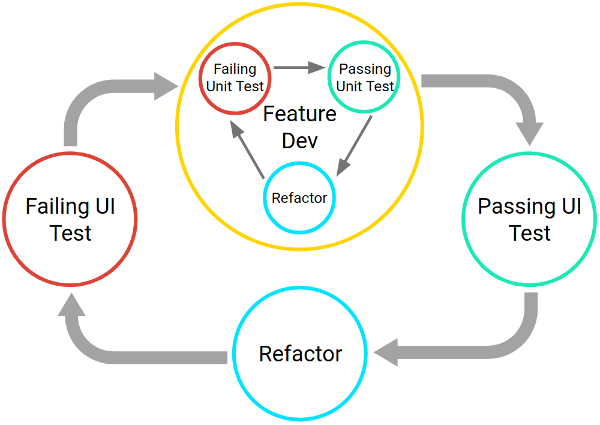
\includegraphics[width=0.5\textwidth]{./google_testing.png}
	\caption[The two cycles associated with iterative, test-driven development]{The two cycles associated with iterative, test-driven development\footnotemark}
	\label{fig_google_testing}
\end{figure}
\footnotetext{\url{https://developer.android.com/images/training/testing/testing-workflow.png}}

Google also defines three types of test categories: (see figure~\ref{fig_google_pyramid})

\begin{figure}[htb]
	\centering
	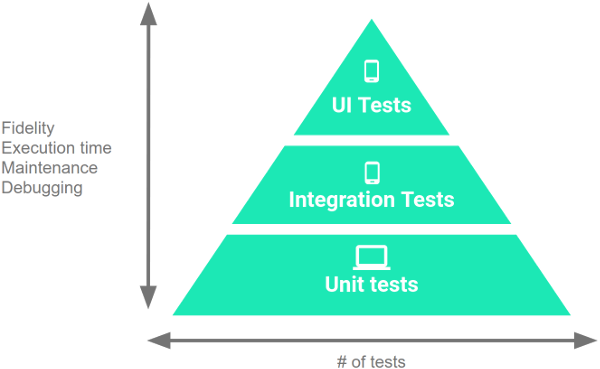
\includegraphics[width=0.5\textwidth]{./pyramid.png}
	\caption[The Testing Pyramid, showing the three categories of tests that should be included in an app's test suite]{The Testing Pyramid, showing the three categories of tests that should be included in an app's test suite\footnotemark}
	\label{fig_google_pyramid}
\end{figure}
\footnotetext{\url{https://developer.android.com/images/training/testing/pyramid.png}}

\begin{itemize}
	\item \textbf{Unit tests - Small tests} \\ 
	These kind of tests validate the behavior of a feature on an atomic level and are highly focues. Around 70\% of the test base should consist of small test, typical frameworks are JUnit, Mockito and PowerMock.
	
	\item \textbf{Integration tests - Medium tests} \\ 
	The next level of testing are the medium/integration tests which are testing the integration of either different level of the the stack within a module or of different modules. The recommendation is to have around 20\% of tests for integration, the toolchain provides Robolectric for this.
	
	\item \textbf{UI tests - Large tests} \\ 
	On top of the testing setup are the large tests, the UI tests. They are used to test end-to-end flows including the interaction of the user with the app through multiple stack level and modules. UI tests are usually very long running flows which have a high ressource impact. It is recommended to have 10\% UI Test, Google provides Espresso and UI Automator on the tool side.
\end{itemize}

For a more detailed overview of the different test size see~\ref{fig_google_test_sizes}.

\begin{figure}[htb]
	\centering
	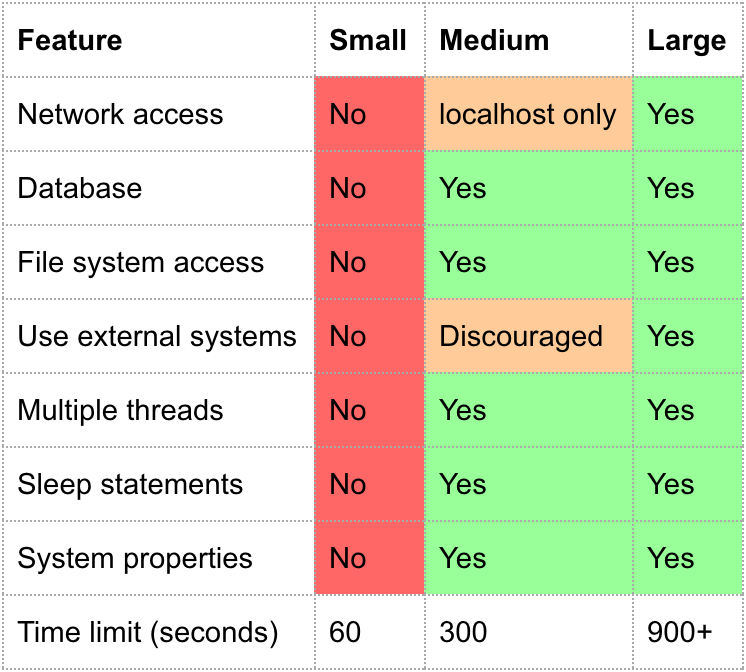
\includegraphics[width=0.5\textwidth]{./test_sizes.png}
	\caption[Test Sizes]{Test Sizes\footnotemark}
	\label{fig_google_test_sizes}
\end{figure}
\footnotetext{\url{https://testing.googleblog.com/2010/12/test-sizes.html}}

Additional to the different test types and sizes, there are also two types of tests based on the environment where they have to be executed:

\begin{itemize}
	\item Normal \textbf{tests}\\
	are executed by the local machine and the JVM and do not require any dependencies to the Android OS. Test resources are located under \texttt{test}.
	\item \textbf{Instrumentation test} \\
	need for execution a mobile device and have a dependency to the Android OS. This device can be physical, virtual (by the Emulator) or simulated (by Roboelectric). Test resources are located under \texttt{androidTest}.
\end{itemize}

Based on this overview of testing classification, the following subsections will give an overview of the tools provided by Google to cover those different levels:

\subsubsection{JUnit, Mockito \& AndroidJUnit4}
The standard JUnit\footnote{\url{https://junit.org/junit4/}} framework is the most obvious solution to build unit tests and is together with Mockito available for use in Android (with JUnit version 4). It is possible to access Android resources within an unit test by configuring gradle with \texttt{unitTests.includeAndroidResources}.

It is further possible to write instrumented JUnit tests by using the \textbf{\texttt{AndroidJUnit4}} test runner (on which e.g. Espresso and UIAutomator relay on). In order to isolate the execution of these tests and to minimize possible shared states between those runs, there is the Android Test Orchestrator\footnote{\url{https://developer.android.com/training/testing/junit-runner}} available.

\subsubsection{Robolectric}
Robolectric\footnote{\url{http://robolectric.org/}} is a framework for unit and integration testing without relaying on a emulator or physical device - instead it uses a simulated device by wrapping the Android framework. This way it can provide far more faster test executions than with instrumentation tests.

\subsubsection{Espresso}
Espresso\footnote{\url{https://developer.android.com/training/testing/espresso}} provides instrumented UI tests with a relatively simple API to use. Next to standard situation with handling UI components, it is able to handle WebViews, idling resources, intents and even multi processes.
Bundled with the \textit{AndroidStudio} comes also the \textbf{Espresso Test Recorder} which simplifies the automatic creation by a great extend - by simply recording an use case.

\subsubsection{UI Automator}
The UI Automator\footnote{\url{https://developer.android.com/training/testing/ui-automator}} framework provides functionality for cross-app UI testing, including interaction between user apps and system apps (e.g. opening the setting menu or app launcher). It further lets tests access hardware functionality such as pressing the Back, Home or Menu buttons or using the volume buttons.

\subsubsection{Android Jetpack Test}

At the I/O18 it the new Android Jetpack component "Android Test"\footnote{\url{https://developer.android.com/training/testing/}} was announced, which aims at unifying the different tools and framework together in one center API within the \textit{AndroidX} package.
At the time of writting this paper, the following tools are fully integrated: Espresso, UI Automator and AndroidJUnitRunner. Robolectric got a major update (v4) for the integration with AndroidX, but is no finished yet.

\begin{mdframed}[style=InfoBox,align=center]
	\textbf{Note:} Google recently (I/O18) also announced "Project Nitrogen" which intents to remove any restrictions of tests to runtime environment - but there are no further information available at the time of writing this paper.
\end{mdframed}

\subsubsection{Outside of the Google ecosystem}

Of course there are many more testing frameworks and tools out there which are not in a direct relation to Google and are not in the standard toolchain. Some well-known examples are:

\begin{itemize}
	\item Appium\footnote{\url{http://appium.io/}}
	\item Detox\footnote{\url{https://github.com/wix/detox}}
	\item Calabash\footnote{\url{http://calaba.sh/}}
	\item screenshot-tests-for-android\footnote{\url{https://facebook.github.io/screenshot-tests-for-android/}}
\end{itemize}



